\chapter{Hammerstein}
W modelu Hammersteina wprowadziłem nieliniowość na wejściu rozmywając sygnał sterujący. W przypadku następników liniowych było to pięć zbiorów rozmytych, natomiast w przypadku następników nieliniowych w postaci sinusa hiperbolicznego, były to już tylko trzy zbiory. Podjąłem próbę z dwoma zbiorami i jest to możliwe, natomiast czas jaki należy poświęcić na dostrajanie modelu bardzo się wydłuża, a za cel postawiłem sobie dostrojenie modelu z następnikami liniowymi i nieliniowymi w podobnym czasie i udało się spełnić to założenie.

\newpage

\section{Następniki liniowe}
Po lepszym zapoznaniu się z Fuzzy Logic Toolbox postanowiłem wykorzystać oferowane przez to narzędzie funkcje. Zbudowałem model rozmyty:

\begin{lstlisting}[style=Matlab-editor]
function linearFuzzy(obj)
U_center = linspace(obj.U_min, obj.U_max, 5);
obj.linear_fis = sugfis('Name', 'Linear_Hammerstein',...
			'Type', 'sugeno');
obj.linear_fis = addInput(obj.linear_fis, [obj.U_min obj.U_max],...
			'Name', 'U_linear');
            
% Definiowanie funkcji przynależności (gaussmf)
for i = 1:length(U_center)
   obj.linear_fis = addMF(obj.linear_fis, 'U_linear', 'gaussmf',...
			[12, U_center(i)]);
end
            
% Definiowanie wyjścia i początkowych następników (a_i * u + b_i)
obj.linear_fis = addOutput(obj.linear_fis, [obj.U_min obj.U_max],...
				'Name', 'U_fuzzy');
            
% Współczynniki (a_i, b_i) następników
a_param = [0.7895 0.8982 1.0933 1.0489 1.2034];
b_param = [0.0001 0.0002 0.0001 0 0.001];
            
% Dodanie reguł TS w postaci liniowej
for i = 1:length(U_center)
   obj.linear_fis = addMF(obj.linear_fis, 'U_fuzzy', 'linear',...
			[a_param(i), b_param(i)]);
end
            
% Reguły Takagi-Sugeno: [inputMF, outputMF, weight]
ruleList = [1 1 1 1;  % Reguła 1: wejście MF1 -> wyjście Out1
            2 2 1 1;  % Reguła 2: wejście MF2 -> wyjście Out2
            3 3 1 1;  % Reguła 3: wejście MF3 -> wyjście Out3
            4 4 1 1;  % Reguła 4: wejście MF4 -> wyjście Out4
            5 5 1 1]; % Reguła 5: wejście MF5 -> wyjście Out5
            
% Dodanie reguł do systemu
obj.linear_fis = addRule(obj.linear_fis, ruleList);
end
\end{lstlisting}

Następniki modelu liniowego były postaci:

\begin{equation}
\begin{array}{c}
\text{Jeśli } u \text{ jest } U^1 \text{ to } u^1_{fuzzy}=a^1u+b^1 \\[1.5ex]
\text{Jeśli } u \text{ jest } U^2 \text{ to } u^2_{fuzzy}=a^2u+b^2 \\[1.5ex]
\text{Jeśli } u \text{ jest } U^3 \text{ to } u^3_{fuzzy}=a^3u+b^3 \\[1.5ex]
\text{Jeśli } u \text{ jest } U^4 \text{ to } u^4_{fuzzy}=a^4u+b^4 \\[1.5ex]
\text{Jeśli } u \text{ jest } U^5 \text{ to } u^5_{fuzzy}=a^5u+b^5 \\[1.5ex]
\end{array}{c}
\end{equation}

\newpage

Zbiory rozmyte rozmieściłem równomiernie na całym zakresie wartości sterowania:

\begin{lstlisting}[style=Matlab-editor]
U_center = linspace(obj.U_min, obj.U_max, 5);
\end{lstlisting}

\noindent Zbadałem trzy kształty funkcji przynależności: \verb+gaussmf+, \verb+gbellmf+ oraz \verb+sigmf+, jednak szybko się okazało, że otrzymywane wyniki nie różnią się w sposób znaczący, a w przypadku funkcji \verb+gaussmf+ potrzeba najmniej parametrów, żeby dobrze zdefiniować taki zbiór, dlatego w przyjąłem tylko taki kształt funkcji przynależności modyfikując jedynie parametry $\sigma$ oraz $\mu$ odpowiadające wariancji oraz wartości średniej. Zbiory rozmyte prezentują się następująco:

\begin{figure}[h!]
\centering
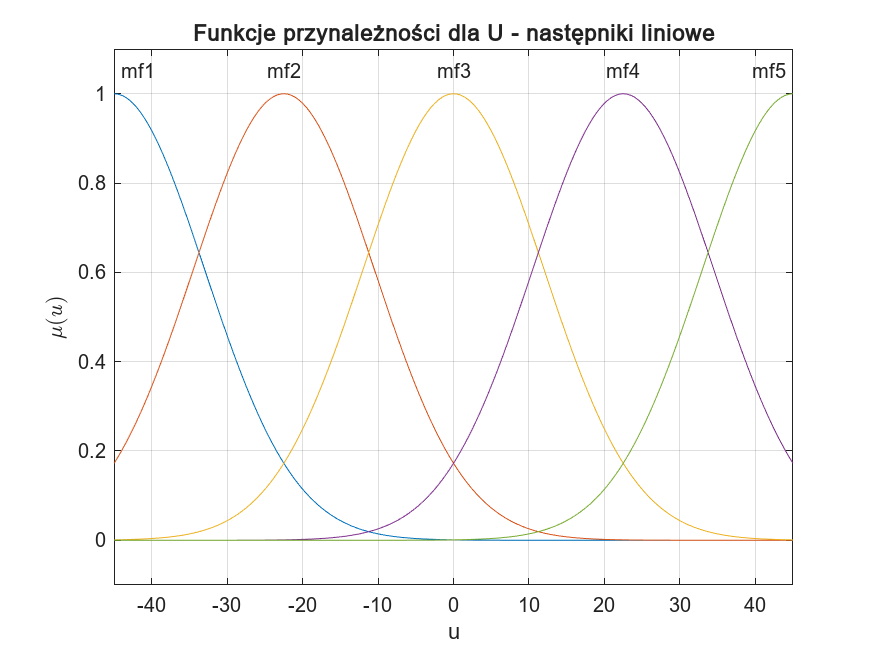
\includegraphics[width=\textwidth]{pictures/HammersteinfuzzySets_liniowe}
\caption{Zbiory rozmyte - model Hammersteina z następnikami liniowymi.}
\end{figure}

\newpage

\section{Następniki nieliniowe}
W przypadku następników hiperbolicznych zdecydowałem się na taką postać:

\begin{equation}
\begin{array}{c}
\text{Jeśli } u \text{ jest } U^1 \text{ to } u^1_{fuzzy}=a^1\sinh \left({\frac{u}{b^1}}\right) \\
\text{Jeśli } u \text{ jest } U^2 \text{ to } u^2_{fuzzy}=a^2\sinh \left({\frac{u}{b^1}}\right) \\
\text{Jeśli } u \text{ jest } U^3 \text{ to } u^3_{fuzzy}=a^3\sinh \left({\frac{u}{b^3}}\right) \\
\end{array}
\end{equation}

\noindent Było to podyktowane kształtem funkcji $\sinh$ i faktowi, że funkcja ta rośnie wykładniczo. Okazało się, że kluczową rolę odgrywa tutaj parametr normalizujący, tj. $b^i$. Jego wartość pozwoliła dobrze modelować wartości sterowania zarówno z niskiego, średniego, jak i wysokiego przedziału. 

\begin{lstlisting}[style=Matlab-editor]
function nonlinearFuzzy(obj)
U_center = linspace(obj.U_min, obj.U_max, 3);
obj.nonlinear_fis = sugfis('Name', 'Nonlinear_Hammerstein',...
			'Type', 'sugeno');
obj.nonlinear_fis = addInput(obj.nonlinear_fis,...
			[obj.U_min obj.U_max], 'Name', 'U_linear');
            
% Definiowanie funkcji przynależności (gaussmf)
for i = 1:length(U_center)
   obj.nonlinear_fis = addMF(obj.nonlinear_fis, 'U_linear',...
			'gaussmf', [20, U_center(i)]);
end
            
% Definiowanie wyjścia i początkowych następników (a_i * u + b_i)
obj.nonlinear_fis = addOutput(obj.nonlinear_fis,...
			[obj.U_min obj.U_max], 'Name', 'U_fuzzy');

% Początkowe współczynniki (a_i, b_i)
a_param = [60.5 50.7 83.5];
b_param = [80 50 75];
            
% Dodanie reguł TS w postaci liniowej
for i = 1:length(U_center)
   obj.nonlinear_fis = addMF(obj.nonlinear_fis, 'U_fuzzy',...
			'linear', [a_param(i), b_param(i)]);
end
            
% Reguły Takagi-Sugeno: [inputMF, outputMF, weight]
ruleList = [1 1 1 1;  % Reguła 1: wejście MF1 -> wyjście Out1
	    2 2 1 1;  % Reguła 2: wejście MF2 -> wyjście Out2
            3 3 1 1];  % Reguła 3: wejście MF3 -> wyjście Out3
            
% Dodanie reguł do systemu
obj.nonlinear_fis = addRule(obj.nonlinear_fis, ruleList);
end
\end{lstlisting}

\newpage

Funkcje przynależności dla modelu Hammersteina z następnikami hiperbolicznymi przedstawiłem na Rys. \ref{HammersteinfuzzySets_nieliniowe}.

\begin{figure}[h!]
\centering
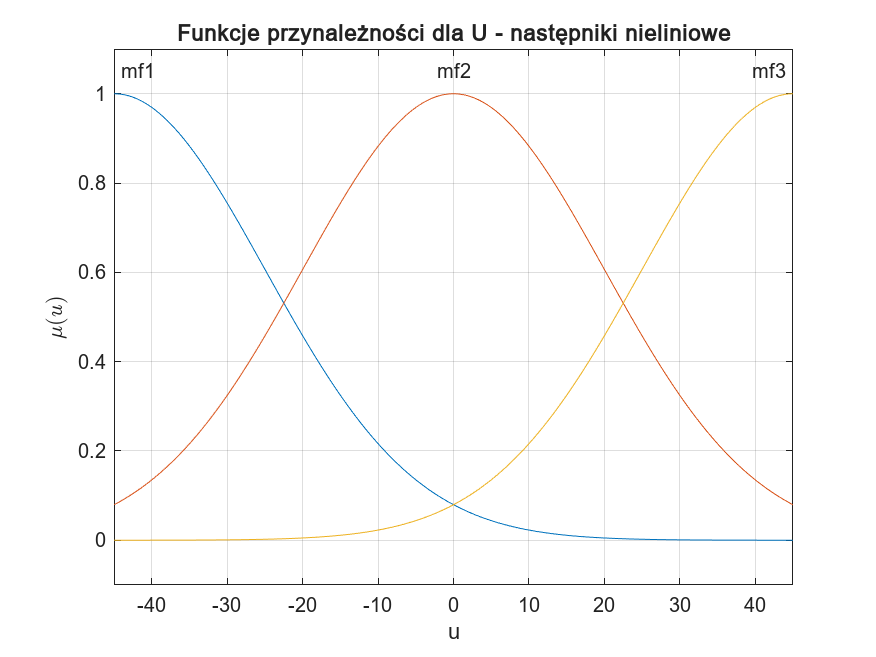
\includegraphics[width=\textwidth]{pictures/HammersteinfuzzySets_nieliniowe}
\caption{Zbiory rozmyte - model Hammersteina z następnikami nieliniowymi.}
\label{HammersteinfuzzySets_nieliniowe}
\end{figure}
